% !TEX root = tracking.tex
\section{Introduction}
 Currently there is a great interest both in research and industry to find methods of fast path planning for autonomous quadrotors and other vehicles. These vehicles must be able to plan and execute a path in real-time without violating safety constraints. This is a very difficult challenge: the need for fast planning is generally at odds with the need for maintaining safety. In order to achieve real-time planning for any environment with static obstacles, researchers typically must use highly simplified model dynamics or kinematics, resulting in a tracking error between the planned path and the true high-dimensional system. This concept is illustrated in Figure \ref{fig:chasing}, where the path was planned using a simplified model (player 1), but the real vehicle (player 2) cannot follow this path exactly. In addition, most current planners do not consider the effect of external disturbance (e.g. wind) on the resulting tracking error. This tracking error due to the simplified dynamics and lack of disturbances can lead to unsafe situations in which the planned path may be safe, but the actual vehicle trajectory crashes into an obstacle or other unsafe region.

We propose precomputing a bound on the possible tracking error between the path planned by the simplified model and the true high-dimensional vehicle dynamics. We compute this by using Hamilton Jacobi reachability analysis to analyze a capture-avoid game in relative coordinates between the true high-dimensional vehicle dynamics and a 'virtual' vehicle that represents the simplified model. Additional external disturbances can be included in this analysis. The result is a mapping from the current relative state to the largest possible tracking error between the two systems over the time period (or for all time, if the game converges). This set captures all deviations due to nonlinearities and disturbance in the true system, and can be thought of as a "safety bubble" around the simplified model (i.e. the path planner). We can prove that \textcolor{red}{statement of proof}. The set also provides a look-up table to determine the optimal control required for the true vehicle to remain as close as possible to the simplified model.

\begin{figure}
	\centering
	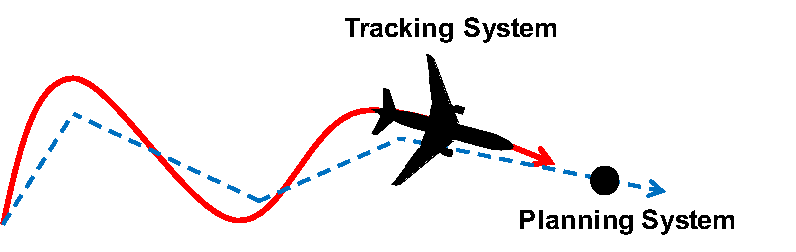
\includegraphics[width=0.47\textwidth]{fig/chasing}
	\caption{\textcolor{red}{filler image about quadrotors chasing each other}}
	\label{fig:chasing}
\end{figure}

We can couple this precomputed set with any path planner or model-predictive control (MPC) that uses the simplified dynamics or kinematics. As the path is being planned using the simplified model, the true vehicle will use the relative state between itself and the current state of the path to a) update the safety bubble and b) look up the optimal control that will minimize tracking error. We can guarantee safety for the path planner by augmenting all encountered obstacles by the safety bubble.

In this paper we demonstrate the method by computing a capture-avoid game between a 10-dimensional quadrotor model and a linear 3D constant-velocity model. We then plan a path through an environment using RRT, while using the precomputed set to determine the safety bubble and optimal control of the 10D system. \textcolor{red}{state results}